\documentclass[12pt]{article}

\usepackage[margin=1in]{geometry}
\usepackage{enumitem}
%\usepackage{forest}
\usepackage{dirtree}
\usepackage{fontawesome5}
\usepackage[utf8]{inputenc}
\usepackage{multicol}
\usepackage[T1]{fontenc}
\usepackage{tabularx}
\usepackage{fancyhdr}
\usepackage{titlesec}
\usepackage{lmodern}
\usepackage{helvet}
\usepackage[hidelinks, breaklinks=true]{hyperref}
\usepackage[svgnames]{xcolor}
\usepackage[table]{xcolor}
\usepackage[framemethod=tikz]{mdframed}
\usepackage[customcolors]{hf-tikz}
\usepackage[most]{tcolorbox}
\usetikzlibrary{shadows}
\usepackage{tgheros}
\renewcommand{\familydefault}{\sfdefault}
\usepackage{listings}
\usepackage[spanish]{babel} 
\usepackage{xcolor,graphicx}
\usepackage{float}
\graphicspath{ {./diagramas/} }
\usepackage{tikz}
\usetikzlibrary{arrows,shapes,positioning,shadows,trees}
%%%%%%%%%%%%%%%%%%%%%%%%%%%%%%%%%%%%%%%%%
% colors
\definecolor{softpurple}{RGB}{145,105,160}
\definecolor{antiquefuchsia}{RGB}{95,60,110}
\titleformat{\section}
  {\color{antiquefuchsia}\normalfont\Large\bfseries}
  {\thesection}{1em}{}

\titleformat{\subsection}
  {\color{antiquefuchsia}\normalfont\large\bfseries}
  {\thesubsection}{1em}{}

\titleformat{\subsubsection}
  {\color{antiquefuchsia}\normalfont\normalsize\bfseries}
  {\thesubsubsection}{1em}{}
%%%%%%%%%%%%%%%%%%%%%%
% Mis comandos
\newcounter{recordatorioCounter}
\newcommand{\recordatorio}{%
  \stepcounter{recordatorioCounter}% avanza el contador
  \textbf{\textcolor{antiquefuchsia}{Recordatorio \therecordatorioCounter : }}%
}
\newcommand{\pb}[1]{\textcolor{softpurple}{\textbf{#1}}}



\lstdefinestyle{mystyle}{
    backgroundcolor=\color{antiquefuchsia!23},   
    commentstyle=\color{codegreen},
    keywordstyle=\color{magenta},
    numberstyle=\tiny\color{codegray},
    stringstyle=\color{codepurple},
    basicstyle=\ttfamily\footnotesize,
    breakatwhitespace=false,         
    breaklines=true,                 
    captionpos=b,                    
    keepspaces=true,                 
    numbers=left,                   
    numbersep=5pt,                  
    showspaces=false,                
    showstringspaces=false,
    showtabs=false,                  
    tabsize=2
}

\lstset{style=mystyle}

% Icono Carpeta
\newcommand{\foldericon}{\faFolderOpen~}

\definecolor{foldercolor}{RGB}{255, 193, 7}
\definecolor{pdfcolor}{RGB}{220, 53, 69}
\definecolor{readmecolor}{RGB}{40, 167, 69}

\renewcommand{\foldericon}{\textcolor{foldercolor}{\faFolder}}
\newcommand{\pdficon}{\textcolor{pdfcolor}{\faFilePdf}}
\newcommand{\txticon}{\textcolor{txtcolor}{\faFileAlt}}
\newcommand{\zipicon}{\textcolor{gray}{\faFileArchive}}



% Set up fancy header/footer
\pagestyle{fancy}
\fancyhead[LO,L]{UNAM}
\fancyhead[RO,R]{\textit{\textsc{Proyecto 1}}}   
\fancyfoot[LO,L]{Facultad De Ciencias, 2027-I}
\fancyfoot[CO,C]{\thepage}
\fancyfoot[RO,R]{Modelado y Programación}
\renewcommand{\headrulewidth}{0.4pt}
\renewcommand{\footrulewidth}{0.4pt}
%%%%%%%%%%%%%%%%%%%%%%

\newdimen\digitwidth
\settowidth\digitwidth{0}
\def~{\hspace{\digitwidth}}

% Cambiar color de secciones
\titleformat{\section}
  {\color{antiquefuchsia}\normalfont\Large\bfseries}
  {\thesection}{1em}{}

\titleformat{\subsection}
  {\color{antiquefuchsia}\normalfont\large\bfseries}
  {\thesubsection}{1em}{}

\titleformat{\subsubsection}
  {\color{antiquefuchsia}\normalfont\normalsize\bfseries}
  {\thesubsubsection}{1em}{}

% Cambiar color de ítems en listas numeradas
\setlist[enumerate]{label=\textcolor{antiquefuchsia}{\arabic*.}, left=1.5em}
\setlist[itemize]{label=\textcolor{antiquefuchsia}{\alph*}, left=1.5em}
\setlist[itemize]{label=\textcolor{antiquefuchsia}{\textbullet}, left=1.5em}


\begin{document}
\begin{titlepage}
\begin{center}

\textsc{\huge\uppercase{Universidad Nacional Autónoma De México}}\\[0.5cm]	

{\huge \uppercase{Facultad de Ciencias, 2027-I} \\[0.5cm] }
{\huge \uppercase{Modelado y Programación} \\[0.5cm] }

%%% Título
\rule{\linewidth}{0.4pt}\\[0.7em]
{ \color{antiquefuchsia} \textsc{\Large Proyecto 1:}} \\[0.7em] 
 \textit{\Large Chat: Servidor - Cliente}
 \\[0.1em] 
 \rule{\linewidth}{0.4pt}\\[0.7em]

{\color{antiquefuchsia} 
\textsc{\Large Morales Galván María Paola}}\\[0.7em]
  \textit{\Large 323073406\\[0.5em] }
  \textit{\Large 28/09/2026}    
 \\[0.1em] 
\rule{\linewidth}{0.4pt}\\[2em]


\color{black!80!black}{\large \uppercase{\textsc{ Profesor:}}}\\[0.25cm]

\begin{tabular}{l}
\large 	Canek Peláez Valdés \\[0.4cm]
\end{tabular}

\large \uppercase{Ayudante de Teoría:}\\[0.2cm]
\centering
\begin{tabular}{l}

\large Cynthia Lizbeth Sánchez Urbano \\[0.4cm]
\end{tabular}

\large \uppercase{Ayudante de Laboratorio:}\\[0.2cm]
\centering
\begin{tabular}{l}

\large Miriam Torres Bucio\\[0.4cm]
\end{tabular}

\vfill

\end{center}
\end{titlepage}

\section*{Resumen}

En este proyecto se diseñó e implementó un sistema de comunicación distribuido en tiempo real bajo la arquitectura cliente-servidor[cite: 1]. La solución se compone de un servidor desarrollado en Golang, encargado del control de concurrencia mediante \textit{goroutines} y la gestión de conexiones de red, y un cliente desarrollado en C\# orientado a la interacción desde la línea de comandos[cite: 1]. Ambos componentes se comunican mediante sockets sobre el protocolo TCP, utilizando tramas serializadas en formato JSON para la transferencia estructurada de mensajes, respuestas y notificaciones[cite: 1]. El sistema permite el intercambio de mensajes privados, difusiones grupales y la administración de salas independientes[cite: 1]. Cabe destacar que esta implementación se desarrolló con fines estrictamente académicos para la asignatura de Modelado y Programación, por lo que omite protocolos de seguridad o cifrado en la transmisión, y los datos presentados en el reporte son de carácter puramente ilustrativo[cite: 1].

\section*{Introducción}

El proyecto aborda el diseño e implementación de un sistema de comunicación en tiempo real distribuido bajo el modelo cliente-servidor. El propósito fundamental es desarrollar una plataforma funcional de chat en consola que gestione conexiones concurrentes, sincronización de estados y un protocolo de mensajería.

\subsubsection*{Objetivos del Proyecto}

\pb{Objetivo General:}
\begin{itemize}
    \item Diseñar e implementar un sistema distribuido de mensajería cliente-servidor tolerante a fallos, capaz de gestionar múltiples conexiones concurrentes y facilitar el intercambio de información estructurada en tiempo real.
\end{itemize}

\pb{Objetivos Específicos:}
\begin{itemize}
    \item Desarrollar un servidor de red capaz de aceptar y administrar múltiples clientes de forma simultánea, asociando a cada uno una unidad de ejecución independiente sin interferir con los demás usuarios.
    \item Implementar un cliente interactivo que permita al usuario enviar mensajes, unirse a salas y recibir notificaciones del servidor asíncronamente en tiempo real.
    \item Implementar un protocolo en formato JSON para normar las solicitudes, respuestas y notificaciones entre ambos componentes.
    \end{itemize}

\subsubsection*{Presentación de Componentes}

El sistema se compone de dos aplicaciones independientes pero estrechamente acopladas por su protocolo de red:
\begin{itemize}
    \item \pb{Servidor (\textit{Golang}):} Encargado de la gestión de conexiones TCP, el control de concurrencia y el almacenamiento de datos en memoria (usuarios activos, invitaciones y salas de chat).
    \item \pb{Cliente (\textit{C\#}):} Captura la entrada del usuario, construye las solicitudes correspondientes y despliega las notificaciones entrantes sin bloquear la interacción.
    \item \pb{Entorno de Construcción (\textit{Meson}):} Sistema de gestión encargado de compilar la aplicación cliente de forma automatizada.
\end{itemize}

Al tratarse de un desarrollo enfocado en el modelado de sistemas concurrentes el proyecto no incluye mecanismos de autenticación o seguridad en el canal de transmisión.


\section*{Analisis y Diseño (Modelo)}

En esta seción desglosaremos como se hizo el analisis y diseño del proyecto

Utilizaremos el siguiente protocolo para el proyecto:

\subsubsection*{Solicitudes del cliente}

  \begin{itemize}
  \item \pb{IDENTIFY:} Para identificar al usuario con el servidor, con la propiedad \hyperlink{param:username}{\textit{username}}
  \item \pb{STATUS:} Cambia el estado de un usuario por (ACTIVE, AWAY o BUSY), con la propiedad \hyperlink{param:status}{\textit{status}}
  \item \pb{USERS:} Solicita la lista de usuarios en el chat
  \item \pb{TEXT:} Manda un mensaje en privado a un usuario, con las propiedades \hyperlink{param:username}{\textit{username}}, \hyperlink{param:text}{\textit{text}}
  \item \pb{PUBLIC\_TEXT:} Manda un mnesaje a todos los usuarios en el chat, con la propiedad \hyperlink{param:text}{\textit{text}}
  \item \pb{NEW\_ROOM:} Crea un cuarto privado, con la propiedad \hyperlink{param:roomname}{\textit{roomname}}
  \item \pb{INVITE:} Invita usuarios al cuarto, con las propiedades \hyperlink{param:roomname}{\textit{roomname}}, \hyperlink{param:usernames}{\textit{usernames}}
  \item \pb{JOIN\_ROOM:} Une al usuario al cuarto siempre y cuando haya sido invitado previamente, con la propiedad \hyperlink{param:roomname}{\textit{roomname}}
  \item \pb{ROOM\_USERS:} Solicita la lista de usuarios en un cuarto, con la propiedad \hyperlink{param:rgoomname}{\textit{roomname}}
  \item \pb{ROOM\_TEXT:} Manda un mensaje dentro de un cuarto, con las propiedades \hyperlink{param:roomname}{\textit{roomname}}, \hyperlink{param:text}{\textit{text}}
  \item \pb{LEAVE\_ROOM:} Solicita dejar un cuarto, con la propiedad \hyperlink{param:roomname}{\textit{roomname}}
  \item \pb{DISCONNECT:} Desconecta al usuario del chat
  \end{itemize}

\subsubsection*{Notificaciones del servidor}

\begin{itemize}
  \item \pb{RESPONSE:} Respuesta directa a una solicitud del cliente, con las propiedades \hyperlink{param:operation}{\textit{operation}}, \hyperlink{param:result}{\textit{result}}, \hyperlink{param:extra}{\textit{extra}}
  \item \pb{NEW\_USER:} Notifica que se unio un nuevo usuario al chat, con la propiedad \hyperlink{param:username}{\textit{username}}
  \item \pb{NEW\_STATUS:} Notifica que algun usuario actualizó su estado a (ACTIVE, AWAY o BUSY), con las propiedades \hyperlink{param:username}{\textit{username}}, \hyperlink{param:status}{\textit{status}}
  \item \pb{USER\_LIST:} Regresa la lista de usuarios del chat, con la propiedad \hyperlink{param:users}{\textit{users}}
  \item \pb{TEXT\_FROM:} Notifica que algun usuaio mando un mensaje en privado, con las propiedades \hyperlink{param:username}{\textit{username}}, \hyperlink{param:text}{\textit{text}}
  \item \pb{PUBLIC\_TEXT\_FROM:} Notifica que algun usuario mando un mensaje al chat grupal, con las propiedades \hyperlink{param:username}{\textit{username}}, \hyperlink{param:text}{\textit{text}}
  \item \pb{JOINED\_ROOM:} Notifica que un usuario se unio a un cuarto, con las propiedades \hyperlink{param:roomname}{\textit{roomname}}, \hyperlink{param:username}{\textit{username}}  
  \item \pb{ROOM\_USER\_LIST:} Regresa la lista de usuarios en un cuarto, con las propiedades \hyperlink{param:roomname}{\textit{roomname}}, \hyperlink{param:users}{\textit{users}}
  \item \pb{ROOM\_TEXT\_FROM:} Notifica que algun usuario mando un mensaje a un cuarto, con las propiedades \hyperlink{param:roomname}{\textit{roomname}}, \hyperlink{param:username}{\textit{username}}, \hyperlink{param:text}{\textit{text}}
  \item \pb{LEFT\_ROOM:} Notifica que un usuario abandono un cuarto, con las propiedades \hyperlink{param:roomname}{\textit{roomname}}, \hyperlink{param:username}{\textit{username}} 
  \item \pb{DISCONNECTED:} Notifica que un usuario se desconecto del chat, con la propiedad \hyperlink{param:username}{\textit{username}} 
  \end{itemize}

\subsubsection*{Respuestas del servidor}
  
  \begin{itemize}
  \item \pb{SUCCESS:} Indica que se ejecuto la acción con exito
  \item \pb{USER\_ALREADY\_EXISTS:} Indica que el nombre de usuario ya existe en el servidor
  \item \pb{NO\_SUCH\_USER:} Indica que el usuario no existe en el chat
  \item \pb{ROOM\_ALREADY\_EXISTS:} Indica que ya existe un cuarto con el nombre
  \item \pb{NO\_SUCH\_ROOM:} Indica que el cuarto no existe
  \item \pb{NOT\_INVITED:} Indica que no has sido invitado al cuarto
  \item \pb{NOT\_JOINED:} Indica que el usuario no se ha unido al cuarto
  \item \pb{NOT\_IDENTIFIED:} Indica que el usuario no se ha identificado
  \end{itemize}

\subsubsection*{Propiedades}

  \begin{itemize}
  \item \hypertarget{param:username}{\pb{username:}} Nombre de usuario del cliente
  \item \hypertarget{param:status}{\pb{status:}} Estado del cliente
  \item \hypertarget{param:text}{\pb{text:}} Mensaje que el cliente quiere enviar
  \item \hypertarget{param:roomname}{\pb{roomname:}} Nombre del cuarto
  \item \hypertarget{param:usernames}{\pb{usernames:}} Nombre de los usuarios
  \item \hypertarget{param:users}{\pb{users:}} Lista de usuarios
  \item \hypertarget{param:operation}{\pb{operation:}} Solicitud que se intento realizar
  \item \hypertarget{param:result}{\pb{result:}} Resultado de la solicitud
  \item \hypertarget{param:extra}{\pb{extra:}} Información extra, usualemte el nombre de usuario o sala
  \end{itemize}

\subsection*{Análisis}

El proyecto consiste en el desarrollo de un sistema de chat en tiempo real. Este problema se puede descomponer en dos partes fundamentales: un servidor capaz de gestionar múltiples clientes de forma simultánea y un cliente capaz de conectarse de manera independiente a dicho servidor. Ambos componentes presentan una dependencia mutua estricta para garantizar el funcionamiento del sistema. Para lograr esto, es imprescindible que cada cliente conectado disponga de su propio hilo o unidad de ejecución concurrente en el servidor, permitiendo procesar distintas acciones simultáneamente.

Por un lado, el servidor debe cumplir con las siguientes funciones clave:

\begin{itemize}
    \item Recibir y gestionar conexiones entrantes.
    \item Mantener la concurrencia activa entre conexiones sin interferir con la operación de otros clientes.
    \item Almacenar y administrar la información de los clientes y las salas en memoria.
    \item Recibir e interpretar mensajes entrantes en formato JSON.
    \item Construir y enviar mensajes de respuesta y notificación en formato JSON.
    \item Ejecutar las acciones solicitadas por cada cliente de manera aislada.
    \item Manejar los posibles errores y fallos de comunicación de forma limpia sin interrumpir el servicio.
\end{itemize}

A partir de estas responsabilidades, se establece que el servidor debe aceptar todas las conexiones válidas. En caso de recibir una conexión inválida o corrupta, debe desconectarla inmediatamente tras detectar el error, sin que esto afecte el comportamiento ni la estabilidad del sistema. El servidor debe mantener la conexión activa con el cliente hasta que este solicite explícitamente su desconexión o hasta que ocurra un error irrecuperable en el canal de red. Mantener la conexión implica procesar correctamente cada solicitud del cliente, emitiendo las respuestas e iterando las notificaciones correspondientes a los demás usuarios.

Es un requisito fundamental que el servidor sea tolerante a fallos e "inmortal", lo que significa que, independientemente de las solicitudes malformadas, la conducta de los clientes o los errores puntuales en las conexiones, el servidor debe continuar operando para el resto de los usuarios conectados. Por último, debe ser capaz de administrar múltiples clientes concurrentes sin incurrir en bloqueos mutuos (deadlocks) ni pérdida de información.

Por otro lado, el cliente debe cumplir con las siguientes responsabilidades:

\begin{itemize}
    \item Establecer la conexión con el servidor a partir de la dirección IP y el puerto proporcionados.
    \item Escuchar continuamente los mensajes enviados por el servidor y las peticiones ingresadas por el usuario.
    \item Interpretar las acciones solicitadas por el usuario desde la interfaz de comandos.
    \item Construir y enviar mensajes en formato JSON hacia el servidor.
\end{itemize}

Dado que el usuario no debe escribir mensajes JSON manualmente, el cliente debe interpretar las órdenes ingresadas por el usuario, transformarlas y construir la estructura JSON correspondiente antes de transmitirla. Asimismo, debe ser capaz de enviar solicitudes y recibir notificaciones o respuestas de forma simultánea, gestionando esta asincronía de manera robusta para evitar fallos en la aplicación. Finalmente, todas las notificaciones recibidas desde el servidor deben ser formateadas y desplegadas al usuario de una manera intuitiva y legible.

Ambos componentes (cliente y servidor) deben acordar un esquema coherente de codificación y decodificación de mensajes JSON para evitar la lectura de parámetros inválidos; por ejemplo, si el servidor envía un valor de tipo cadena (*string*), el cliente debe decodificarlo explícitamente bajo el mismo tipo de dato.

\subsection*{Diseño}

La elección de \textbf{Golang} para la implementación del servidor se fundamenta en su modelo de concurrencia nativo basado en \textit{goroutines}, el cual permite gestionar múltiples conexiones TCP simultáneas con un consumo mínimo de recursos, sumado a la simplicidad del paquete \texttt{net} para la creación de \textit{listeners} y sockets.

Por su parte, el lenguaje \textbf{C\#} para el desarrollo del cliente se seleccionó debido a sus librerías de red nativas, las cuales permiten crear y administrar sockets de forma directa e intuitiva, ofreciendo además herramientas integradas para la serialización y deserialización de datos entre JSON u objetos de C\#. Adicionalmente, se integró el sistema de construcción \textbf{Meson} al cliente debido a su facilidad en la administración de dependencias y a que permite definir reglas de compilación claras en su archivo de configuración (\texttt{meson.build}), generando el ejecutable del proyecto sin necesidad de ejecutar comandos complejos.

A continuación, se detalla la comunicación e interacción entre el servidor y el cliente según lo establecido en la etapa de análisis.

\begin{figure}[H]
    \centering
    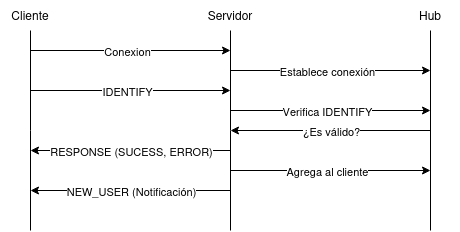
\includegraphics[width=0.85\textwidth]{Uso.png}
    \caption{Diagrama de conexión e identificación del cliente.}
    \label{fig:conexion}
\end{figure}

Como se observa en el diagrama, el cliente inicia el proceso intentando conectarse al servidor. Una vez establecida la conexión, el cliente debe identificarse enviando la solicitud \textit{IDENTIFY}. Si la identificación es válida, el servidor registra al usuario y emite la notificación \textit{NEW\_USER} al resto de los clientes conectados. Cabe destacar que todos los mensajes recibidos por el servidor siguen un mismo ciclo de procesamiento: recepción, validación, interpretación y ejecución. Si alguno de estos pasos falla, el cliente en cuestión es desconectado para prevenir fallos globales y preservar la ejecución del servidor.

El siguiente diagrama ejemplifica el funcionamiento y las estructuras internas del servidor:

\begin{figure}[H]
    \centering
    \includegraphics[width=0.85\textwidth]{servidor.png}
    \caption{UML del servidor.}
    \label{fig:servidor}
\end{figure}

Como se observa, el servidor mantiene dos propiedades principales representadas como mapas/diccionarios:
\begin{itemize}
    \item \pb{Usuarios:} Almacena el nombre de usuario como clave y una referencia a la estructura \texttt{Cliente} como valor.
    \item \pb{Salas:} Almacena el nombre de la sala como clave y una referencia a la estructura \texttt{Sala} correspondiente.
\end{itemize}
Estas estructuras permiten preservar el registro global de todos los usuarios y salas existentes en el sistema.

Por su parte, la abstracción del \textbf{Cliente} en el servidor se compone de tres propiedades:
\begin{itemize}
    \item \pb{Usuario:} Nombre identificador elegido por el cliente.
    \item \pb{Conexión:} Referencia al socket o identificador del cliente dentro de la red.
    \item \pb{Estado:} Valor perteneciente a la enumeración de estados permitidos, cuyo valor predeterminado al conectarse es \texttt{ACTIVE}.
\end{itemize}

Las \textbf{Salas} contienen tres propiedades fundamentales:
\begin{itemize}
    \item \pb{Nombre:} Nombre identificador de la sala.
    \item \pb{Clientes:} Diccionario que asocia el nombre del usuario (*string*) con su respectiva referencia de \texttt{Cliente}.
    \item \pb{Invitados:} Diccionario con la misma estructura que el de clientes, utilizado para llevar el control de los usuarios que han sido invitados a la sala.
\end{itemize}

La estructura genérica de los \textbf{Mensajes} dispone de 10 propiedades que corresponden exactamente a los campos definidos en el protocolo JSON, garantizando una estructura homogénea para la transferencia de datos.

Adicionalmente, se implementaron tres enumeraciones principales (\texttt{TIPO}, \texttt{RESPUESTA} y \texttt{ESTADO}). Esta decisión de diseño permite que, al recibir un mensaje en formato JSON, el sistema pueda validar e identificar de forma limpia si la operación o el contenido es válido.

A continuación, se ejemplifica el funcionamiento interno del cliente:

\begin{figure}[H]
    \centering
    \includegraphics[width=0.85\textwidth]{cliente.png}
    \caption{UML del cliente.}
    \label{fig:cliente}
\end{figure}

Como se puede observar, el cliente mantiene tres propiedades principales:
\begin{itemize}
    \item \pb{Usuario:} Nombre del usuario identificado.
    \item \pb{Estado:} Estado actual del usuario.
    \item \pb{Conexión:} Instancia de la conexión por socket con el servidor.
\end{itemize}

Para la administración del estado local, la abstracción del entorno del cliente conserva:
\begin{itemize}
    \item Una referencia al cliente.
    \item Un diccionario de clientes (clave: \textit{string}, valor: \textit{Estado}).
    \item Un diccionario de salas (clave: \textit{string}, valor: \textit{Lista de cadenas}).
    \item Una lista de invitaciones recibidas.
\end{itemize}
Lo anterior evita la necesidad de solicitar constantemente la lista completa de usuarios al servidor, permitiendo además acceder localmente a la información de las salas a las que se pertenece o a las que se ha sido invitado.

Al igual que en el servidor, los mensajes en el cliente contienen las propiedades definidas por el protocolo para asegurar el formato de las tramas serializadas. Se incluyen las enumeraciones \texttt{Tipo}, \texttt{Respuesta} y \texttt{Estado} para validar las tramas entrantes y garantizar el correcto armado de los JSON salientes.

\section*{Implementación}

En esta sección se describen las tecnologías específicas, bibliotecas, mecanismos de sincronización y métodos clave que hacen funcional la arquitectura del sistema de chat.

\subsection*{Tecnologías Utilizadas}

\begin{itemize}
    \item \pb{Servidor (Golang):} Implementado en Go utilizando su librería nativa \texttt{net} para el manejo de conexiones TCP sobre sockets, \texttt{encoding/json} para la serialización y deserialización de mensajes, y el paquete \texttt{sync} para el control de concurrencia.
    \item \pb{Cliente (C\#):} Desarrollado en C\# (.NET) utilizando \texttt{System.Net.Sockets} para la gestión del socket de red, \texttt{System.Text.Json} para el parseo de estructuras de mensajes y hilos/tareas asíncronas (\texttt{Task.Run}) para no bloquear la consola durante la lectura.
    \item \pb{Administración del Proyecto (Meson):} Se incorporó el sistema de construcción Meson para definir el flujo de compilación del cliente de C\# a través del archivo \texttt{meson.build}.
\end{itemize}

\subsection*{Detalles y Métodos Clave del Servidor (Golang)}

El servidor se diseñó para procesar clientes de forma concurrente protegiendo las estructuras globales en memoria (\texttt{Usuarios} y \texttt{Salas}) mediante cerrojos de exclusión mutua (\texttt{sync.RWMutex}).

\begin{itemize}
    \item \pb{Método Temporal:} Controla la conexión inicial de un cliente antes de que este se identifique. Escucha el socket entrante y valida que el primer mensaje sea un comando \texttt{IDENTIFY}. Si el nombre de usuario ya está registrado en la estructura global o el mensaje es inválido, emite la respuesta de error y cierra el socket inmediatamente, evitando el desperdicio de recursos.
    \item \pb{Métodos de Gestión de Memoria (AgregarCliente, EliminarCliente, AgregarSala, EliminarSala):} Métodos encargados de la modificación de las estructuras de mapas en el servidor. Dado que en Go no es seguro modificar un mapa mientras se iteran sus elementos desde múltiples \textit{goroutines}, estos métodos encierran las operaciones entre bloques \texttt{Lock()} y \texttt{Unlock()} del cerrojo \texttt{RWMutex}, asegurando modificaciones atómicas.
    \item \pb{Gestión de Conexiones Activas:} Por cada conexión aceptada en el socket principal, el servidor lanza una nueva \textit{goroutine} que atiende de forma asíncrona la lectura continua de tramas JSON enviadas por dicho cliente.
\end{itemize}

\subsection*{Detalles y Métodos Clave del Cliente (C\#)}

El cliente gestiona la asincronía entre la lectura del teclado por parte del usuario y la recepción de notificaciones de red enviadas por el servidor.

\begin{itemize}
    \item \pb{Método Temporal:} Maneja la rutina de conexión del cliente. Solicita los datos de red (IP y puerto), establece la conexión socket mediante \texttt{TcpClient} y envía el paquete de identificación \texttt{IDENTIFY}. Al recibir una respuesta exitosa (\texttt{SUCCESS}), inicializa las estructuras locales y solicita automáticamente la lista actualizada de usuarios (\texttt{USERS}).
    \item \pb{Método EscuchaCliente:} Se ejecuta en el hilo principal de la aplicación. Mantiene un bucle continuo capturando la entrada ingresada por el usuario en la terminal, traduce la orden a su representación JSON equivalente usando el protocolo acordado y la transmite por el socket.
    \item \pb{Método EscuchaServidor:} Corre en un hilo secundario asíncrono (\texttt{Task.Run}). Permanece a la espera de bytes en el socket, deserializa las tramas JSON entrantes y despliega las notificaciones (\texttt{TEXT\_FROM}, \texttt{NEW\_USER}, \texttt{ROOM\_TEXT\_FROM}, etc.) formateadas en la consola sin interrumpir la escritura activa del usuario.
\end{itemize}

\section*{Conclusiones}

El desarrollo de este proyecto me permitió integrar de forma práctica los conceptos de la programación concurrente, el diseño de sistemas distribuidos bajo el modelo cliente-servidor y la manipulación de sockets de red. La utilización de \textit{goroutines} y la simplicidad del paquete \texttt{net} considero que fueron un asierto para la construcción del servidores, ya que me facilitaron la atención simultánea de múltiples clientes mediante hilos. Asimismo, logre notar la importancia de aplicar un control estricto de exclusión mutua mediante cerrojos de lectura y escritura para proteger las estructuras compartidas en memoria.

Por otro lado, en la implementación del cliente, la ejecución asíncrona mediante tareas en segundo plano en C\# permitió procesar las notificaciones del servidor en tiempo real sin congelar ni bloquear la captura de comandos ingresados desde la terminal. De igual forma, la integración del sistema de construcción Meson simplificó de manera notable la administración de dependencias y el flujo de compilación del cliente.

En cuanto a las dificultades encontradas durante el desarrollo, uno de los mayores retos radicó en la gestión precisa de los cerrojos de exclusión mutua (\texttt{sync.RWMutex}) para prevenir la aparición de interbloqueos (\textit{deadlocks}) al acceder y modificar concurrentemente las estructuras. Asimismo, la correcta implementación del protocolo representó un reto significativo, ya que requirió garantizar que los mensajes en formato JSON fueran serializadas y deserializadas de manera simétrica y sin ambigüedades.

\section*{Bibliografía}

\begin{enumerate}
    \item The Go Programming Language Documentation. \textit{Package net: Sockets TCP, Listeners y manejo de conexiones de red}. Disponible en: \url{https://pkg.go.dev/net}
    \item The Go Programming Language Documentation. \textit{Package sync: Cerrojos Mutex (RWMutex) y control de concurrencia}. Disponible en: \url{https://pkg.go.dev/sync}
    \item The Go Programming Language Documentation. \textit{Package encoding/json: Serialización y deserialización de datos}. Disponible en: \url{https://pkg.go.dev/encoding/json}
    \item Microsoft .NET Documentation. \textit{System.Net.Sockets Namespace: Manejo de sockets y conexiones TCP en C\#}. Disponible en: \url{https://learn.microsoft.com/en-us/dotnet/api/system.net.sockets}
    \item Microsoft .NET Documentation. \textit{System.Text.Json Namespace: Serialización y mapeo de objetos JSON en C\#}. Disponible en: \url{https://learn.microsoft.com/en-us/dotnet/standard/serialization/system-text-json-overview}
    \item Microsoft .NET Documentation. \textit{Asynchronous programming with async and await / Task.Run in C\#}. Disponible en: \url{https://learn.microsoft.com/en-us/dotnet/csharp/asynchronous-programming/}
    \item The Meson Build System Documentation. \textit{Meson Build System Reference Manual y sintaxis de meson.build}. Disponible en: \url{https://mesonbuild.com/}
    \item IETF RFC 793. \textit{Transmission Control Protocol (TCP) Specification: Asignación de puertos efímeros, estados de conexión y ciclo de vida de sockets}. Disponible en: \url{https://datatracker.ietf.org/doc/html/rfc793}
    \item IETF RFC 8259. \textit{The JavaScript Object Notation (JSON) Data Interchange Format}. Disponible en: \url{https://datatracker.ietf.org/doc/html/rfc8259}
    \item Tanenbaum, A. S., \& Wetherall, D. J. \textit{Redes de Computadoras: Arquitectura Cliente-Servidor y Capa de Transporte}. 5ta Edición, Pearson Education.
\end{enumerate}

\end{document}
